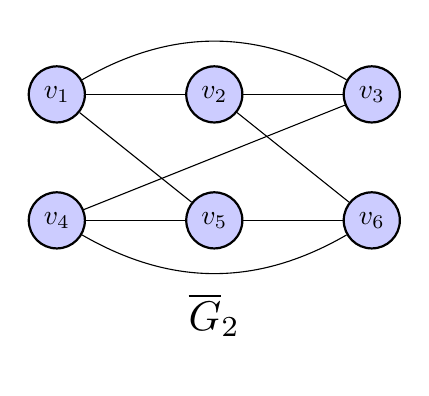
\begin{tikzpicture}
  [scale=.8,auto=left,every node/.style={circle,fill=blue!20,draw=black,thick}]
  
  % Fila superior
  \node (n1) at (0,2) {$v_1$};
  \node (n2) at (2.5,2) {$v_2$};
  \node (n3) at (5,2) {$v_3$};

  % Fila inferior
  \node (n4) at (0,0) {$v_4$};
  \node (n5) at (2.5,0) {$v_5$};
  \node (n6) at (5,0) {$v_6$};

  % Aristas del complemento \overline{G}_2
  % Conexiones dentro de la misma fila
  \draw (n1) to[bend left=30] (n3);
  \draw (n1) -- (n2);
  \draw (n2) -- (n3);
  
  \draw (n4) to[bend right=30] (n6);
  \draw (n4) -- (n5);
  \draw (n5) -- (n6);

  % Conexiones entre filas que faltaban en G_2
  \draw (n1) -- (n5);
  \draw (n2) -- (n6);
  \draw (n3) -- (n4);

  % Etiqueta \overline{G}_2 debajo del grafo
  \node[draw=none, fill=none, scale=1.5] at (2.5,-1.5) {$\overline{G}_2$};

\end{tikzpicture}
